\documentclass[14pt]{extarticle}
% \documentclass[14pt]{article}

% \usepackage[style=authoryear,maxbibnames=9,maxcitenames=2,uniquelist=false,backend=biber,doi=false,url=false]{biblatex}
% \addbibresource{$BIB} % bibtex location
% \renewcommand*{\nameyeardelim}{\addcomma\space} % have comma in parencite
\usepackage{natbib}

\usepackage{xcolor}
\usepackage{amsmath}
\newcommand{\tuple}[1]{ \langle #1 \rangle }
%\usepackage{automata}
\usepackage{times}
\usepackage{ltablex}
\usepackage{tasks}

%%%%%% Template
\usepackage{hyperref}
\hypersetup{colorlinks=true,allcolors=blue}

\usepackage{vmargin}
\setpapersize{USletter}
\setmarginsrb{1.0in}{1.0in}{1.0in}{0.6in}{0pt}{0pt}{0pt}{0.4in}

% HOW TO USE THE ABOVE:
%\setmarginsrb{leftmargin}{topmargin}{rightmargin}{bottommargin}{headheight}{headsep}{footheight}{footskip}
%\raggedbottom
% paragraphs indent & skip:
\parindent  0.3cm
\parskip    -0.01cm

\usepackage{tikz}
\usetikzlibrary{backgrounds}

% hyphenation:
% \hyphenpenalty=10000 % no hyphen
% \exhyphenpenalty=10000 % no hyphen
\sloppy

% notes-style paragraph spacing and indentation:
\usepackage{parskip}
\setlength{\parindent}{0cm}

% let derivations break across pages
\allowdisplaybreaks

\newcommand{\orange}[1]{\textcolor{orange}{#1}}
\newcommand{\blue}[1]{\textcolor{blue}{#1}}
\newcommand{\red}[1]{\textcolor{red}{#1}}
\newcommand{\freq}[1]{{\bf \sf F}(#1)}
\newcommand{\datafreq}[2]{{{\bf \sf F}_{#1}(#2)}}

\def\qqquad{\quad\qquad}
\def\qqqquad{\qquad\qquad}

%%%%%%%%%%%%%%%%%%%%%%%%%%%%%%%%%%%%%%%%%%%%%%%%%%%%%%%%%%%%%%%%%%%%%%%%%%%%%%%%
%%%%%%%%%%%%%%%%%%%%%%%%%%%%%%%%%%%%%%%%%%%%%%%%%%%%%%%%%%%%%%%%%%%%%%%%%%%%%%%%

% fill-in-blank question style, found in https://tex.stackexchange.com/a/505089

\usepackage{ifthen}
\usepackage{tocloft}
\usepackage{exercise}
% \usepackage{xcolor}

% Set the Show Answers Boolean
\newboolean{showAns}
\setboolean{showAns}{false}
\newcommand{\showAns}{\setboolean{showAns}{true}}

% The length of the Answer line
\newlength{\answerlength}
\newcommand{\anslen}[1]{\settowidth{\answerlength}{#1}}

% ans command that indicates space for an answer or shows the answer in red
\newcommand{\ans}[1]{\settowidth{\answerlength}{\hspace{2ex}#1\hspace{2ex}}%
    \ifthenelse{\boolean{showAns}}%
        {\textcolor{red}{\underline{\hspace{2ex}#1\hspace{2ex}}}}%
        {\underline{\hspace{\answerlength}}}}%

\newcommand{\details}[1]{\settowidth{\answerlength}{#1}%
    \ifthenelse{\boolean{showAns}}%
        {\\ \textcolor{blue}{#1}}%
        {}}%

% Formatting how multiple choices Questions are formated.
\settasks{label=(\Alph*), label-width=30pt}


% Some commands for the Exercise Question package
\renewcommand{\QuestionNB}{\Large\protect\textcircled{\small\bfseries\arabic{Question}}\ }
\renewcommand{\ExerciseHeader}{} %no header
\renewcommand{\QuestionBefore}{3ex} %Space above each Q
\setlength{\QuestionIndent}{8pt} % Indent after Q number


% To create the list of answers with tocloft...
\newcommand{\listanswername}{Answers}
\newlistof[Question]{answer}{Answers}{\listanswername}

% Creates a TOC for Answers
\newcounter{prevQ}
\newcommand{\answer}[1]{\refstepcounter{answer}%
\ans{#1}%
\ifnum\theQuestion=\theprevQ%
        \addcontentsline{Answers}{answer}{\protect\numberline{}#1}% don't include the Q number
        \else%
        \addcontentsline{Answers}{answer}{\protect\numberline{\theQuestion}#1}%
        \setcounter{prevQ}{\value{Question}}%
        \fi%
        }%

% \hyphenpenalty=10000 % no hyphen
% \exhyphenpenalty=10000 % no hyphen
\sloppy              % hyphen

\newcommand{\HRule}{\rule{\linewidth}{0.5mm}}
\newcommand{\Hrule}{\rule{\linewidth}{0.3mm}}

%tocloft formatting listofanswers
\renewcommand{\cftAnswerstitlefont}{\bfseries\large}
\renewcommand{\cftanswerdotsep}{\cftnodots}
\cftpagenumbersoff{answer}
\addtolength{\cftanswernumwidth}{10pt}

\makeatletter% since there's an at-sign (@) in the command name
\renewcommand{\@maketitle}{%
  \parindent=0pt% don't indent paragraphs in the title block
  \centering
  {\Large \bfseries\textsc{\@title}} \\
  \vspace{5pt}
  {\large \textit{\@author}} \\
  \HRule \\
  \vspace{1em}
}
\makeatother% resets the meaning of the at-sign (@)


\title{ECON 2002.01 Problem Set 4 }
\author{Unit 7 \\
  \vspace{5pt}
    Hui-Jun Chen}


%%%%%%%%%%%%%%%%%%%%%%%%%%%%%%%%%%%%%%%%%%%%%%%%%%%%%%%%%%%%%%%%%%%%%%%%%%%%%%%%
%%%%%%%%%%%%%%%%%%%%%%%%%%%%%%%%%%%%%%%%%%%%%%%%%%%%%%%%%%%%%%%%%%%%%%%%%%%%%%%%
\begin{document}

\maketitle

\showAns
\listofanswer

\begin{Exercise}

\Question (OUP-U7-Q2)
    Consider the demand curve shown in the figure. Suppose that the unit cost (the cost of producing each pound of Cheerios) is C = \$2. Based on the demand curve, which of the following statements is correct?
\answer{C}

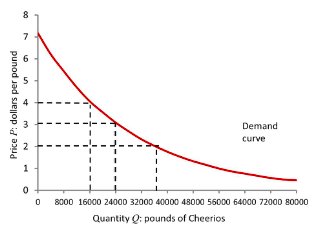
\includegraphics[width=\textwidth]{../QuestionBankImage/OUP-U7-Q1-01.png}

\begin{tasks}(1)
    \task The total revenue when Q = 24,000 is \$48,000.
        \details{When Q = 24,000, P = 3. Then the total revenue is P × Q = 3 × 24,000 = \$72,000. \$48,000 is the total cost.}
    \task The total cost when P = 4 is \$64,000.
        \details{When P = 4, Q = 16,000. Then the total cost is C × Q = 2 × 16,000 = \$32,000. \$64,000 is the total revenue.}
    \task The profit when P = 3 is \$24,000.
        \details{When P = 3, Q = 24,000. Then the profit is (P – C) × Q = (3 – 2) × 24,000 = \$24,000.}
    \task The profit when Q = 16,000 is \$64,000.
        \details{When Q = 16,000, P = 4. Then the profit is (P – C) × Q = (4 – 2) × 16,000 = \$32,000. \$64,000 is the total revenue.}
\end{tasks}


\Question (OUP-U7-Q6)
Which of the following statements regarding the marginal rate of substitution (MRS) and the marginal rate of transformation (MRT) of a profit-maximising firm is correct?
\answer{A}
\begin{tasks}(1)
    \task
	The MRS is how much in price you are willing to give up for an incremental increase in the quantity, holding profits constant.
        \details{This is the definition of the MRS. It is the slope of the isoprofit curves.}
    \task The MRT is how much in price the consumers are willing to give up for an incremental increase in the quantity consumed, keeping their utility constant.
        \details{The MRT is how much the firms have to drop the price for an incremental increase in demand. It is the slope of the demand curve.}
    \task If MRT $>$ MRS then firms can increase their profit by increasing output.
        \details{When MRT $>$ MRS, the slope of the demand curve is steeper than the slope of the isoprofit curve that intersects the demand curve. This means that for a unit decrease in output, firms are able to increase the price more than the amount required to keep their profit constant. Therefore to increase profit, they should decrease output.}
    \task The MRT is the slope of the isoprofit curves.
        \details{The MRT is the slope of the demand curve.}
\end{tasks}

\Question (OUP-U7-Q8)
    The table represents market demand Q for a good at different prices P. The firm’s unit cost of production is £70. Based on this information, which of the following is correct?


\includegraphics[width=\textwidth]{../QuestionBankImage/OUP-U7-Q8-01.png}

\answer{C}
\begin{tasks}(1)
    \task
At Q = 200, the firm’s profit is £44,000.
        \details{At Q = 200, profit = (220 – 70) × 200 = £30,000. £44,000 is the total revenue.}
    \task
	The profit-maximising output is Q = 400.
        \details{At Q = 400, profit = (180 – 70) × 400 = £44,000. At Q = 500, profit = (160 – 70) × 500 = £45,000. Therefore Q = 400 is not the profit-maximising output.}
    \task
	The maximum profit that can be attained is £45,000.
        \details{The maximum profit is attained at Q = 500, where profit = (160 – 70) × 500 = £45,000. This can be checked by calculating profits at all P.}

    \task
	The minimum profit that can be attained is £0.
        \details{The firm makes a loss at Q = 1000, where the price is below the unit cost of production}
\end{tasks}

\Question
(OUP-U7-Q11)
    Which of the following statements regarding average cost and marginal cost of a firm is correct?
\answer{D}
\begin{tasks}(1)
    \task
	Average cost is the slope of the total cost curve.
        \details{Average cost is the slope of the ray from the origin to a point on the total cost curve.}
    \task
	Marginal cost is the slope of the average cost curve.
        \details{Marginal cost is the slope of the total cost curve.}
    \task
	Marginal cost is always higher than average cost.
        \details{When average cost decreases with output, marginal cost is lower than the average cost.}
    \task
	When marginal cost equals average cost, the slope of the average cost curve is zero.
        \details{When marginal cost equals average cost, the cost of producing one extra unit of output is the same as the average of the costs of producing all existing outputs. This keeps the average the same, so the average cost curve is horizontal at this point.}
\end{tasks}

\Question
(OUP-U7-Q15)
    The diagram depicts the demand curve of a product. Assume that there are 100 potential buyers who can choose to purchase one unit each. Based on this graph, which of the following statements is correct?
\answer{A}

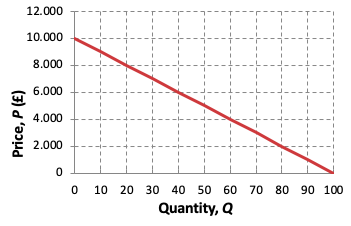
\includegraphics[width=\textwidth]{../QuestionBankImage/OUP-U7-Q15-01.png}
\begin{tasks}(1)
    \task
The diagram demonstrates the Law of Demand.
        \details{The Law of Demand states that when the price is high, demand is low, while when the price is low, demand is high. The downward sloping demand curve clearly demonstrates this.}
    \task
	At an output of 20, the willingness to pay of all 20 consumers who buy the product is £8,000.
        \details{The buyers’ willingness to pay is decreasing in quantity: the first buyer is willing to pay £10,000, while the 20th buyer’s willingness to pay is £8,000.}
    \task
	A quarter of the buyers are not willing to pay more than £2,000 for the product.
        \details{At a price of £2,000 there are only 80 buyers, so one-fifth of the buyers are not willing to pay more than £2,000 for the product.}
    \task
	The firm should sell all 100 units in order to maximise its profits.
        \details{To sell all 100 units, the firm would have to set the price to be £0. The firm can increase its profit by reducing output.	}
\end{tasks}


\Question
(OUP-U7-Q22)
    The figure depicts the demand curve of a firm producing cars, together with its marginal cost, average cost, and isoprofit curves. Based on the figure, which of the following statements is correct?
\answer{C}
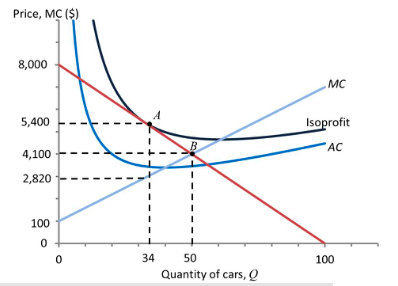
\includegraphics[width=\textwidth]{../QuestionBankImage/OUP-U7-Q22-01.png}

\begin{tasks}(1)
    \task
The consumer surplus in the profit-maximising outcome is \$105,300.
        \details{The profit-maximising outcome is A. The consumer surplus is ½ × (8000 – 5400) × 34 = \$44,200. \$105,300 is the consumer surplus at the Pareto efficient outcome B.}
    \task
	The producer surplus in the Pareto efficient outcome is \$133,960.
        \details{The Pareto-efficient outcome is B. The producer surplus is ½ × (4000 – 100) × 50 = \$100,000. \$133,960 is the producer surplus at the profit-maximising outcome A.}
    \task
	The deadweight loss in the profit-maximising outcome is \$20,640.
        \details{The profit-maximising outcome is A. The deadweight loss is ½ × (5400 – 2820) × (50 – 34) = \$20,640.}
    \task
    	The firm’s profit in the Pareto efficient outcome is \$100,000.
        \details{The Pareto-efficient outcome is B. \$100,000 is the producer surplus at this point. The firm’s profit is producer surplus minus its fixed costs, so is less than \$100,000}
\end{tasks}

\Question

Different from the slide, this question provides a different illustration fo profit maximization problem.
The slide is using $ MR = MC $ to illustrate, while this question is treating profit like utility to consumer, and draw the ``isoprofit curve'', i.e., a contour plot of 3D profit function.

(TEA-U7-Q5)   The following figure depicts a firm’s profit-maximisingchoice at point E, given the market demand curve and the firm’s marginal cost curve. You are given that the firm’s marginal costs are \$400, \$2,960 and \$4,200 at output levels Q = 0, Q* = 32 (point E) and $Q_0= 48$ (point F), respectively. Based on this information, which of the following statements is correct?
\answer{C}
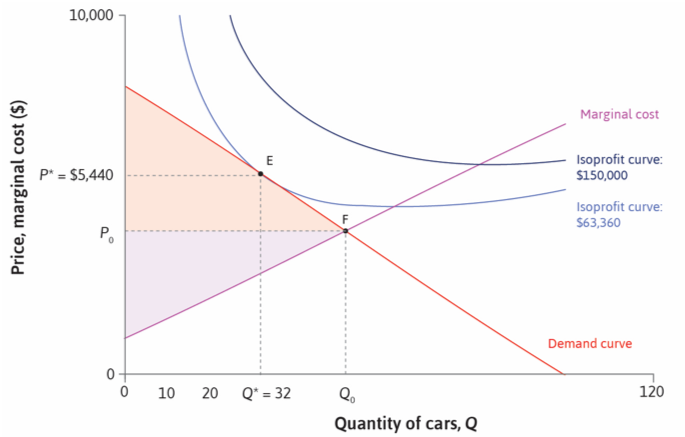
\includegraphics[width=\textwidth]{../QuestionBankImage/TEA-U7-Q5-01.png}

\begin{tasks}(1)
    \task
	The consumer surplus at E is \$41,000.
        \details{The consumer surplus at E is (1/2) x (7920 – 5440) x 32 = \$39,680.}
    \task
	The producer surplus at E is \$126,720.
        \details{The producer surplus at E is (1/2) x (2480 + 5040) x 32 = \$120,320.}
    \task
	The deadweight loss at E is \$19,840.
        \details{The deadweight loss at E is (5440 – 2960) x (48 – 32) x (1/2) = \$19,840.}
    \task
	The gains from trade at E are \$120,320.
        \details{The gains from trade at E are the sum of consumer surplus and producer surplus: CS + PS = 39,680 + 120,320 = \$160,000.	}
\end{tasks}

\Question
(UCL-S16-Q4) Demand faced by a monopolist is Q = 20 – 0.5P. Her marginal cost is 10. Based on this information we can say that:
\answer{C}
\begin{tasks}(1)
    \task
	The optimal production of the monopolist is Q = 15.
        \details{The monopolist will produce until MR = MC. From the demand function, we find that P = 40 - 2Q. Therefore, revenue R is $R = Q \times  P = 40Q - 2Q^2$. Marginal revenue MR is: $dR/dQ = MR = 40 - 4Q$. Because MR = MC, then 40 - 4Q = 10 which implies that Q* = 7.5. So the monopolist will produce 7.5 units.}
    \task
	The price charged by the monopolist is equal to her marginal cost.
        \details{This would be true in case of perfect competition. In this case, the price is obtained through the inverse demand function: P* = 40 - 2Q* = 40 - 2 x 7.5 = 25.}
    \task
	The deadweight loss associated with the monopolist’s choice of price is less than the product of the difference between her price and marginal cost, multiplied by her optimal quantity.
        \details{The deadweight loss (DWL) associated with the monopolist's choice is DWL = (1/2) x ((25 - 10) x (15 - 7.5)) = 56.25. The product of the difference between her price and marginal cost multiplied by her optimal quantity is given by (25 - 10) x 7.5 = 112.5.}
    \task
	The price charged by the monopolist is lower to her marginal cost.
        \details{If the price is lower than marginal cost then she is incur a loss for every unit sold. So this is wrong.}
\end{tasks}

\Question
(ECO-U7-Q5) Consider a firm with fixed costs of production. Which of the following statements about its average cost (AC) and marginal cost (MC) is correct?
\answer{A}
\begin{tasks}(1)
    \task
When $AC = MC$, the AC curve has a zero slope.
        \details{When AC = MC, the cost of an additional unit equals the average cost of all existing units. Therefore, the new AC will be the same and the slope is zero.}
    \task
	When $AC > MC$, the MC curve is downward-sloping.
        \details{The MC curve can be upward-sloping, horizontal, or downward-sloping, irrespective of the relative size of AC and MC.}
    \task
	When $AC < MC$, the AC curve is downward-sloping.
        \details{When $AC < MC$, the cost of an additional unit is greater than the average cost of the existing outputs. So the new AC will be larger. The AC curve is upward-sloping.}
    \task
	The MC curve cannot be horizontal.
        \details{If MC is constant, then the MC curve is horizontal.}
\end{tasks}

\Question
(ECO-U7-Q12) This figure shows the marginal cost and marginal revenue curves for Beautiful Cars. Which of the following statements is correct, based on the information shown?
\answer{D}

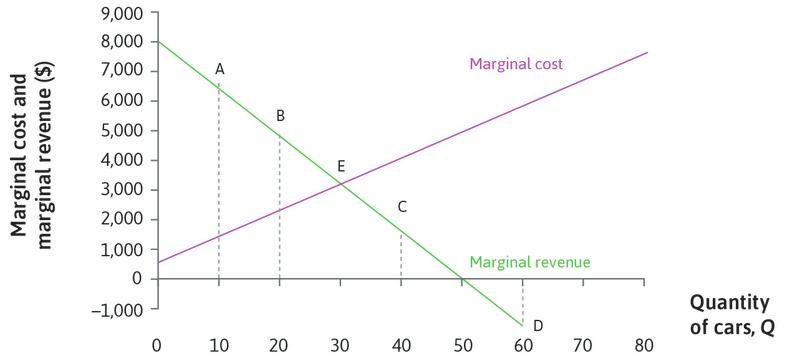
\includegraphics[width=\textwidth]{../QuestionBankImage/ECO-U7-Q12-01.jpg}
\begin{tasks}(1)
    \task
When Q = 40, the marginal cost is greater than the marginal revenue so the firm’s profit must be negative.
        \details{When Q = 40 the marginal cost is greater than the marginal revenue so the marginal profit is negative. This doesn’t mean that profit is negative.}
    \task
	Revenue is greater when Q = 10 than if Q = 20.
        \details{The marginal revenue is greater at Q = 10 than Q = 20. But because the marginal revenue is positive as output increases from 10 to 20, revenue is increasing: it is higher at Q = 20.}
    \task
	The firm would not choose to produce at point E because marginal profit is zero.
        \details{Marginal profit is zero at E. But this is the profit-maximizing point, so the firm will choose it.}
    \task
    	Profit is greater when Q = 20 than when Q = 10.
        \details{At all levels of output up to point E, marginal revenue is greater than marginal cost. So profit increases as output increases—it is higher at Q = 20 than Q = 10.	}
\end{tasks}

\end{Exercise}

\end{document}
